\section{Weil classes and Schoen's subvariety}\label{sec:weil}

In this section $K$ is an imaginary quadratic field with a fixed embedding
$\chi\colon K\to\CC$ and its conjugate $\bar\chi$. Let $A$ be an abelian
variety of Weil type for $K$ of dimension $2n$ (\Cref{ssec:weilfamilies}) on
which $\cO_{K}$ acts, with a polarization class $\eta$ whose Rosati
involution induces complex conjugation on $K$. Endomorphisms act on
cohomology by pull-back, which makes $V=H^{1}(A,\QQ)$ a $K$-vector space of
dimension $2n$, and
\[
  V_{\CC}=V\otimes_{\QQ}\CC=V_{\chi}\oplus V_{\bar\chi},
\]
where $\alpha\in K$ acts on $V_{\chi}$ by $\chi(\alpha)$ and on
$V_{\bar\chi}$ by $\bar\chi(\alpha)$. Each summand has dimension $2n$ and,
because $A$ is of Weil type, meets $H^{1,0}$ and $H^{0,1}$ in subspaces of
dimension $n$. The Weil plane satisfies
\[
  W(A)\otimes\CC=\textstyle\bigwedge^{2n}V_{\chi}\oplus\bigwedge^{2n}V_{\bar\chi}
  \subseteq H^{2n}(A,\CC)
\]
\cite[\S4]{Del82}, and both lines are of type $(n,n)$. We call $A$
\emph{Weil-algebraic} if every class in $W(A)$ is algebraic. Two facts are
used repeatedly. First, an endomorphism $\alpha\in\cO_{K}$ multiplies
$\eta$ by the norm $N(\alpha)=\chi(\alpha)\bar\chi(\alpha)$, since its Rosati
adjoint is $\bar\alpha$; comparing with the action of $\alpha$ on
$\bigwedge^{2}V_{\CC}=\bigwedge^{2}V_{\chi}\oplus(V_{\chi}\otimes
V_{\bar\chi})\oplus\bigwedge^{2}V_{\bar\chi}$ for any $\alpha\notin\QQ$ shows
that $\eta\in V_{\chi}\otimes V_{\bar\chi}$, and hence
\begin{equation}\label{eq:etapower}
  \eta^{k}\in\textstyle\bigwedge^{k}V_{\chi}\otimes\bigwedge^{k}V_{\bar\chi}.
\end{equation}
Second, if $W(A)$ contains one nonzero algebraic class, then $A$ is
Weil-algebraic, by the argument given for $\xi_{s}$ in
\Cref{ssec:weilfamilies}.

The Hodge group $\Hg(A)$ commutes with $K$ and preserves the Riemann form,
so it lies in the unitary group $\U(V,H)$ of the hermitian form $H$ of the
polarization. It fixes the Hodge classes in $W(A)$, on which $\U(V,H)$ acts
through the determinant, so $\Hg(A)\subseteq\SU(V,H)$. We say that $A$ has
\emph{maximal Hodge group} if equality holds.

\subsection{The Hodge ring of a general member}

\begin{proposition}\label{prop:hodgering}
If $\Hg(A)=\SU(V,H)$, then $\Hdg^{k}(A)=\QQ\,\eta^{k}$ for $k\ne n$, and
\[
  \Hdg^{n}(A)=\QQ\,\eta^{n}\oplus W(A).
\]
Moreover $\eta^{n}\cup w=0$ for every $w\in W(A)$.
\end{proposition}

\begin{proof}
The Hodge classes in $H^{2k}(A,\QQ)=\bigwedge^{2k}V$ are the invariants of
$\Hg(A)$ \cite[\S3]{Del82}. Over $\CC$ the group $\SU(V,H)$ becomes
$\mathrm{SL}(V_{\chi})$, acting on $V_{\chi}$ by the standard representation
and on $V_{\bar\chi}$ by its dual, because the Riemann form pairs
$V_{\bar\chi}$ perfectly with $V_{\chi}$. The invariants in
\[
  \textstyle\bigwedge^{2k}V_{\CC}=\bigoplus_{a+b=2k}\bigwedge^{a}V_{\chi}
  \otimes\bigwedge^{b}V_{\chi}^{\vee}
  =\bigoplus_{a+b=2k}\operatorname{Hom}\bigl(\bigwedge^{b}V_{\chi},
  \bigwedge^{a}V_{\chi}\bigr)
\]
form a line in each summand with $a=b$ or $\{a,b\}=\{0,2n\}$, and vanish in
the others, because the representations $\bigwedge^{a}V_{\chi}$, $0\le
a\le2n$, are irreducible and pairwise non-isomorphic except for
$\bigwedge^{0}\cong\bigwedge^{2n}$.\footnote{The representation
$\bigwedge^{a}$ of $\mathrm{SL}_{2n}$ is irreducible with highest weight the
$a$-th fundamental weight for $1\le a\le 2n-1$, and these weights are
distinct; $\bigwedge^{0}$ and $\bigwedge^{2n}$ are trivial.} By
\eqref{eq:etapower} the line for $a=b=k$ contains $\eta^{k}$, which is
nonzero for $k\le2n$ because $\eta^{2n}$ is a positive multiple of the
orientation class. In degree $2n$ the two remaining lines span
$W(A)\otimes\CC$. This proves the first two assertions. By
\eqref{eq:etapower}, $\eta^{n}\cup\bigwedge^{2n}V_{\chi}$ lies in
$\bigwedge^{3n}V_{\chi}\otimes\bigwedge^{n}V_{\bar\chi}=0$, and likewise for
$V_{\bar\chi}$.
\end{proof}

\subsection{What is known}\label{ssec:weilknown}
For $n=1$ the Weil plane lies in $H^{2}$ and \Cref{thm:lef11} applies. For
$n=2$ the hermitian form is split exactly when its discriminant is trivial,
and Floccari and Fu prove that the Weil classes of every Weil fourfold of
discriminant one are algebraic \cite{FF26}. Schoen proves algebraicity for
the Weil fourfolds of trivial discriminant for $\QQ(\sqrt{-3})$ and for the
Weil sixfolds of a family for $\QQ(\sqrt{-3})$ in which his Prym varieties
are dense \cite{Sch88,Sch98}, and for further families of fourfolds
\cite{Sch98}; Koike treats families for $\QQ(\sqrt{-1})$ built in the same
way \cite{Koi04}. Markman's preprint proves algebraicity for every Weil
fourfold and every split Weil sixfold \cite{Mar25a}. Since the Hodge ring of
an abelian variety of dimension at most five is generated by divisor classes
and the Weil classes of its quotients \cite{MZ99}, the fourfold case gives
\st{F2} in dimension at most five. For $2n\ge8$ we know of
no family of Weil type whose general member has maximal Hodge group and on
which the Weil classes are known to be algebraic at every member.

\subsection{Semiregularity}\label{ssec:semireg}
Let $Z$ be a smooth projective variety of dimension $N$ and $\mathcal{E}$ a
coherent sheaf on $Z$, with Atiyah class
$\operatorname{at}(\mathcal{E})\in\operatorname{Ext}^{1}(\mathcal{E},
\mathcal{E}\otimes\Omega^{1}_{Z})$. The \emph{semiregularity map} of
Buchweitz and Flenner is
\[
  \sigma_{\mathcal{E}}\colon\operatorname{Ext}^{2}(\mathcal{E},\mathcal{E})
  \longrightarrow\bigoplus_{q=0}^{N-2}H^{q+2}(Z,\Omega^{q}_{Z}),\qquad
  e\longmapsto\Bigl(\operatorname{tr}\bigl(\operatorname{at}(\mathcal{E})^{q}
  \circ e\bigr)/q!\Bigr)_{q},
\]
and $\mathcal{E}$ is \emph{semiregular} if $\sigma_{\mathcal{E}}$ is
injective \cite{BF03}. A subvariety $Y\subseteq Z$ is semiregular if
$\cO_{Y}$ is.\footnote{Bloch introduced semiregularity for local complete
intersection subvarieties, through a map $H^{1}(Y,N_{Y/Z})\to
H^{p+1}(Z,\Omega^{p-1}_{Z})$ in codimension $p$, and proved the deformation
theorem below in that setting \cite{Blo72}. Buchweitz and Flenner extend
both the map and the theorem to coherent sheaves.} The point of the
definition is the following theorem. If an infinitesimal deformation of $Z$
keeps $\ch(\mathcal{E})$ of Hodge type, the obstruction to deforming
$\mathcal{E}$ along it is sent by $\sigma_{\mathcal{E}}$ to the obstruction
for $\ch(\mathcal{E})$ to stay of Hodge type, which vanishes; injectivity
of $\sigma_{\mathcal{E}}$ then kills the first obstruction.

\begin{theorem}[{Buchweitz--Flenner \cite[Theorem~1.5]{BF03}, after Bloch
\cite{Blo72}}]\label{thm:bf}
Let $f\colon\mathcal{Z}\to T$ be a smooth projective morphism to a connected
complex manifold, let $0\in T$, and let $\mathcal{E}$ be a semiregular
coherent sheaf on $\mathcal{Z}_{0}$. Suppose that over a contractible
neighbourhood of $0$ the flat continuation of every component of
$\ch(\mathcal{E})$ is a Hodge class on every fibre. Then $\mathcal{E}$
extends to a coherent sheaf on $f^{-1}(U)$, flat over $U$, for some open
neighbourhood $U$ of $0$.
\end{theorem}

We return to the split Weil family $\pi\colon\cA\to S$ of
\Cref{ssec:weilfamilies}, with its global section $\xi$ of Weil planes and
the sets $\Sigma_{d}\subseteq\Sigma\subseteq S$ of \Cref{def:sigmad}.

\begin{proposition}\label{prop:semireg}
Let $s_{0}\in S$ and let $\mathcal{E}$ be a semiregular coherent sheaf on
$A=\cA_{s_{0}}$ such that $\ch_{k}(\mathcal{E})\in\QQ\,\eta^{k}$ for $k\ne
n$ and $\ch_{n}(\mathcal{E})=a\,\eta^{n}+w$ with $a\in\QQ$ and $0\ne w\in
W(A)$. Then $\Sigma=S$: the Weil classes are algebraic on every member of
the family.
\end{proposition}

\begin{proof}
The powers of $\eta$ extend to flat sections that are Hodge classes on every
member, and so does $w$, since the Weil planes form a trivial local system
of Hodge classes on $S$ (\Cref{ssec:weilfamilies}). So the hypothesis of
\Cref{thm:bf} holds, and $\mathcal{E}$ extends to a sheaf on
$\pi^{-1}(U)$, flat over $U$, for a contractible open neighbourhood $U$ of
$s_{0}$ in $S^{\mathrm{an}}$. For $t\in U$ its restriction $\mathcal{E}_{t}$
is algebraic by GAGA and has a finite locally free resolution, so
$\ch(\mathcal{E}_{t})$ is algebraic, and it is the flat continuation of
$\ch(\mathcal{E})$. Hence $w_{t}=\ch_{n}(\mathcal{E}_{t})-a\,\eta_{t}^{n}$ is
a nonzero algebraic class in $W(\cA_{t})$, and $t\in\Sigma$. Thus
$U\subseteq\Sigma=\bigcup_{d}\Sigma_{d}$. By the Baire category theorem some
$\Sigma_{d}$ contains a nonempty open subset of $S^{\mathrm{an}}$; it is
Zariski closed by \Cref{lem:sigmaclosed} and $S$ is irreducible, so
$\Sigma_{d}=S$.
\end{proof}

\subsection{Schoen's subvariety}\label{ssec:schoen}
From now on $K=\QQ(\sqrt{-3})$, and $\zeta\in\cO_{K}$ is a primitive cube
root of unity. Let $X$ be a curve of genus $g=n+1\ge3$, let $L\in
\Pic^{0}(X)$ have exact order three, and let $\pi\colon C\to X$ be the
\'etale cyclic triple cover defined by $L$, with covering automorphism
$\sigma$; thus $\pi_{*}\cO_{C}=\cO_{X}\oplus L\oplus L^{2}$, and $C$ has
genus $3g-2$. In $J=J(C)$ put $N=1+\sigma+\sigma^{2}$ and $P=3-N$, and let
$B=P(J)$, the \emph{Prym variety} of the cover, with the polarization $\eta$
induced by the principal polarization of $J$. Since $N^{2}=3N$, we have
$NP=0$ and $P^{2}=3P$; so $P$ is multiplication by $3$ on $B$, and $\sigma$
acts on $B$ with $\sigma^{2}+\sigma+1=0$, which lets $\zeta$ act as $\sigma$.

\begin{lemma}\label{lem:prym}
\begin{enumerate}[label=\textup{(\alph*)}]
\item $B$ is an abelian variety of Weil type for $K$ of dimension $2n$.
\item The hermitian form of $\eta$ is split.
\item For very general $(X,L)$, $B$ has maximal Hodge group.
\end{enumerate}
\end{lemma}

\begin{proof}
(a) By the decomposition of $\pi_{*}\cO_{C}$, the space $H^{0}(C,K_{C})$ is
the sum of $H^{0}(X,K_{X}\otimes L^{j})$, $j=0,1,2$, on which $\sigma^{*}$
acts by the three cube roots of unity. By Riemann--Roch these spaces have
dimensions $g$, $g-1$ and $g-1$, since $L^{j}$ is a nontrivial bundle of
degree zero for $j=1,2$. Let $P'\colon J\to B$ be $P$ with its target
restricted and $\iota\colon B\to J$ the inclusion. Since $P'\iota=3$ and
$P=\iota P'$, pull-back by $P'$ identifies $H^{1,0}(B)$ with the image of
$P^{*}=3-N^{*}$ on $H^{1,0}(J)$, which is the sum of the two nontrivial
eigenspaces. So $\dim B=2(g-1)=2n$, and both embeddings of $K$ occur with
multiplicity $n$.

(b) The Riemann form of $\eta$ is the intersection form $E$ on
$H_{1}(B,\QQ)=P\,H_{1}(C,\QQ)$, and a $K$-subspace is isotropic for the
hermitian form exactly when it is isotropic for $E$. The cover corresponds to
a surjection $\phi\colon H_{1}(X,\ZZ)\to\ZZ/3$. Since $\mathrm{Sp}_{2g}(\ZZ)$
maps onto $\mathrm{Sp}_{2g}(\ZZ/3)$, which is transitive on nonzero vectors,
there is a symplectic basis $a_{1},b_{1},\dots,a_{g},b_{g}$ with
$\phi(x)=\langle x,b_{1}\rangle\bmod 3$; represent it by simple closed
curves in standard position. For $i\ge2$ the curves $a_{i}$ and $b_{i}$ have
trivial monodromy, so each lifts to three disjoint closed curves, permuted by
$\sigma$. Choose lifts $\tilde a_{i}$ and $\tilde b_{i}$ that meet. Then
$E(\sigma^{k}\tilde a_{i},\sigma^{l}\tilde a_{j})=0$ and
$E(\sigma^{k}\tilde a_{i},\sigma^{l}\tilde b_{j})=\delta_{ij}\delta_{kl}$
for $i,j\ge2$. The first relation shows that the $\ZZ[\sigma]$-span of the
classes $P\tilde a_{i}$, $2\le i\le g$, is isotropic. These classes are
$K$-linearly independent: if $\sum_{i}\alpha_{i}P\tilde a_{i}=0$ with
$\alpha_{i}=\sum_{k}c_{ik}\sigma^{k}\in\ZZ[\sigma]$, pairing with
$\sigma^{l}\tilde b_{j}$ gives $3c_{jl}-\sum_{k}c_{jk}=0$ for every $l$, so
$c_{j0}=c_{j1}=c_{j2}$ and $\alpha_{j}$ is a multiple of $N$, which is zero
on $B$. So they span an isotropic subspace of dimension $n=g-1$.

(c) The monodromy of the Prym varieties over the moduli of pairs $(X,L)$ is
an arithmetic subgroup of the unitary group \cite{Loo97}, so by Borel density its Zariski closure contains
$\SU(V,H)$. By Andr\'e's theorem \cite{And92} the connected
monodromy group is contained in the Hodge group of a very general member.
Together with $\Hg(B)\subseteq\SU(V,H)$ this gives equality.
\end{proof}

The pairs $(X,L)$ of genus $g$ have $3g-3=3n$ moduli, while the split Weil
family of $K$ in dimension $2n$ has dimension $n^{2}$. For $n\le3$ Schoen uses these Prym varieties to reach every member
\cite{Sch88,Sch98}. For $n\ge4$ they form a proper subvariety
(\Cref{fig:dims}).

\begin{figure}[t]
\centering
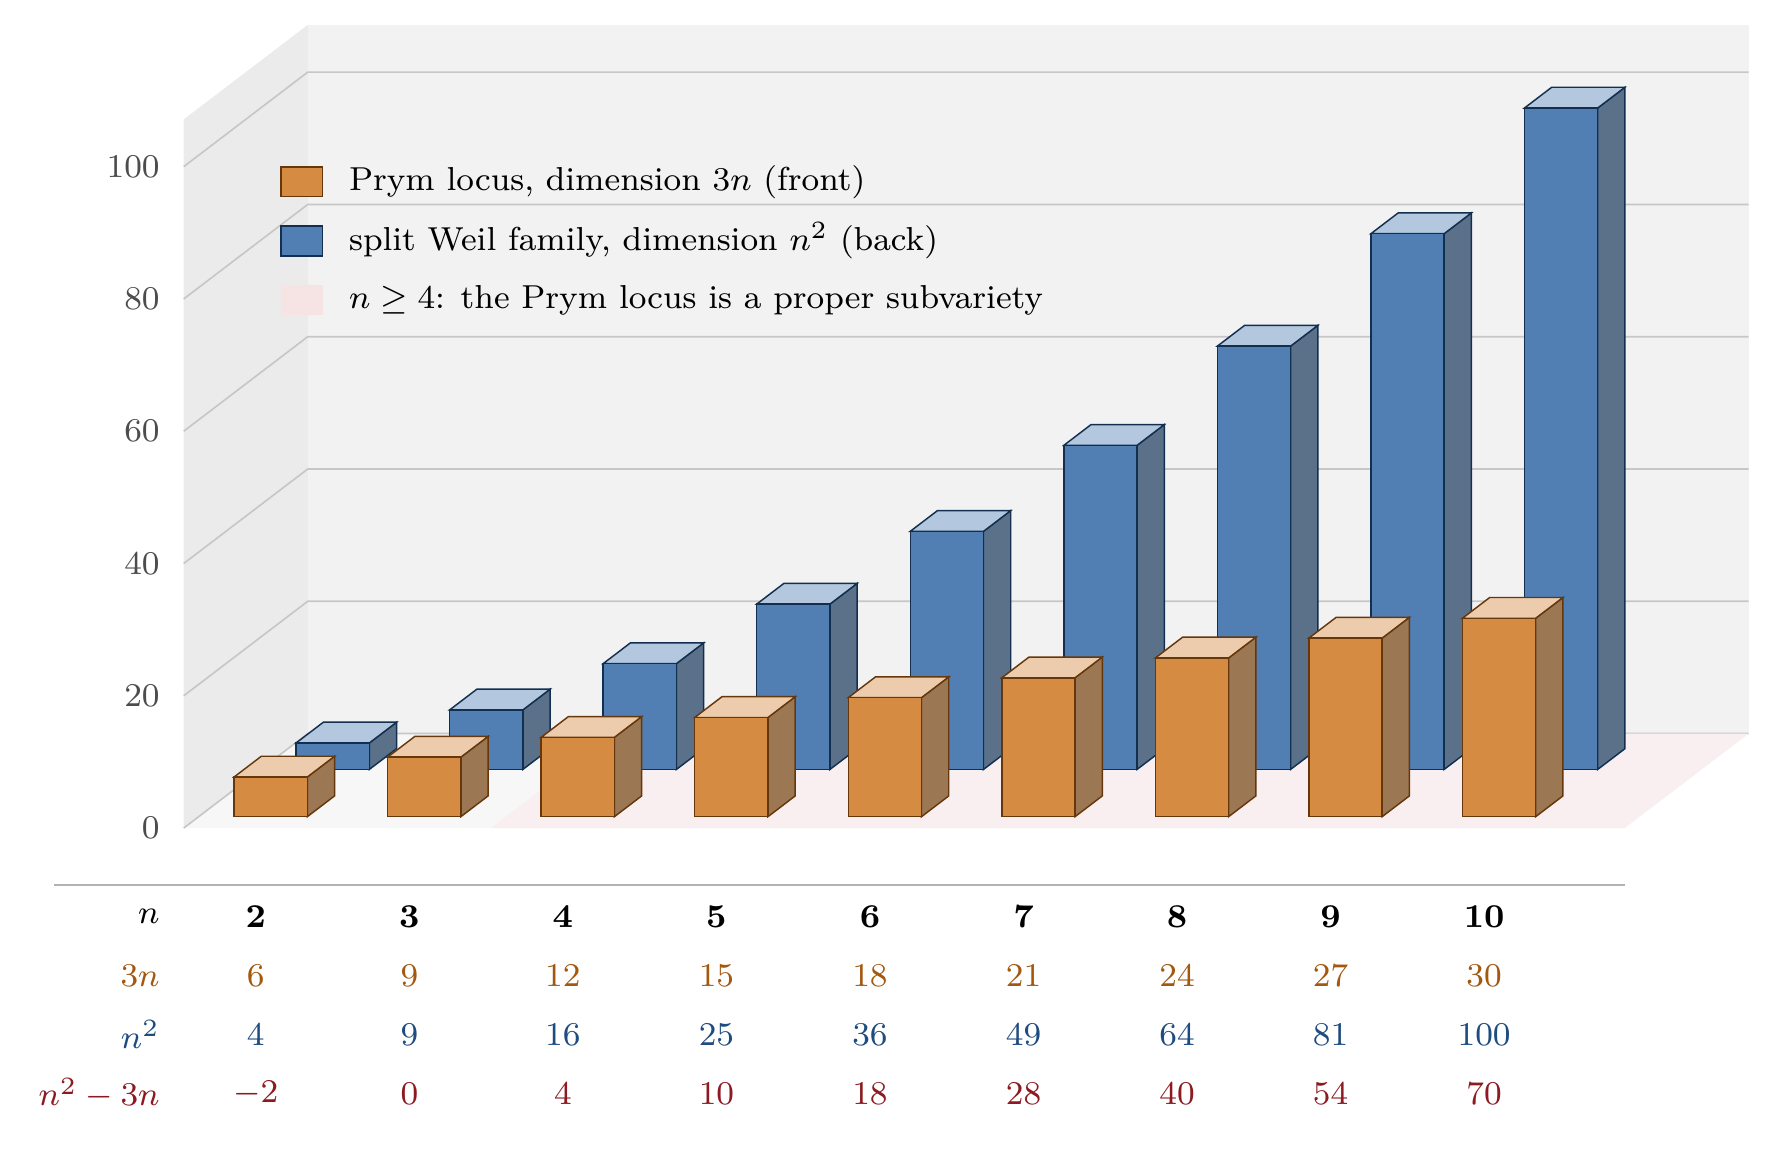
\includegraphics[width=0.9\textwidth]{figures/fig_dims}
\caption{The dimension $3n$ of the locus of Prym varieties of \'etale
cyclic triple covers of curves of genus $n+1$, against the dimension $n^{2}$
of the split Weil family of $\QQ(\sqrt{-3})$ in dimension $2n$. For $n\ge4$
the Prym locus is a proper subvariety, and a semiregular $Y$ would have to
deform in the $n^{2}-3n$ remaining directions.}
\label{fig:dims}
\end{figure}

\emph{The construction.} Let $h=2g-2=2n$. The group
$G=(\ZZ/3)^{h}\rtimes S_{h}$ acts on $C^{h}$ by
$(v,\tau)\cdot(c_{i})_{i}=(\sigma^{v_{i}}c_{\tau^{-1}(i)})_{i}$, and the
quotient is the symmetric product $X^{(h)}$; write $\mu\colon C^{h}\to
X^{(h)}$. The map $\varepsilon(v,\tau)=\sum_{i}v_{i}$ is a homomorphism
$G\to\ZZ/3$, with kernel $G'$. Following Schoen \cite[\S2]{Sch88}, put
\[
  W_{0}=C^{h}/G',\qquad \rho\colon C^{h}\to W_{0},\qquad
  \nu\colon W_{0}\to X^{(h)},
\]
and let $\delta=\sigma\times1\times\dots\times1$, so that $\varepsilon(\delta)
=1$ and $\delta$ induces an automorphism $\bar\delta$ of $W_{0}$ over
$X^{(h)}$.

\begin{lemma}\label{lem:quotient}
\begin{enumerate}[label=\textup{(\alph*)}]
\item No element of $G\setminus G'$ has a fixed point on $C^{h}$. Hence
$\nu$ is a connected \'etale Galois cover with group $\ZZ/3$, generated by
$\bar\delta$.
\item $G$ acts freely on $\mu^{-1}(D)$ for every reduced divisor $D\in
X^{(h)}$.
\item $\mu$ is finite and flat, so $\mu^{-1}$ of a subvariety of pure
dimension $r$ has pure dimension $r$.
\end{enumerate}
\end{lemma}

\begin{proof}
Suppose $(v,\tau)$ fixes $(c_{i})$, so that
$c_{\tau(i)}=\sigma^{v_{\tau(i)}}c_{i}$ for all $i$. Going once around a
cycle $(i_{1},\dots,i_{k})$ of $\tau$ gives $c_{i_{1}}=\sigma^{v_{i_{1}}+
\dots+v_{i_{k}}}c_{i_{1}}$; since $\sigma$ has no fixed points, the sum of
the $v_{i}$ over every cycle is $0$ in $\ZZ/3$, and so is
$\varepsilon(v,\tau)$. This is~(a): $W_{0}$ is connected as a quotient of
$C^{h}$, and $G/G'\cong\ZZ/3$ acts freely on it with quotient $X^{(h)}$. If
moreover the points $\pi(c_{i})$ are distinct, then $\pi(c_{\tau(i)})=
\pi(c_{i})$ forces $\tau=1$, and then $v=0$; this is~(b). The map $C^{h}\to
X^{h}$ is \'etale and $X^{h}\to X^{(h)}$ is a finite map between smooth
varieties of the same dimension, hence flat. By going down for flat maps,
every component of the preimage of a subvariety $Z$ dominates a component of
$Z$, and the fibres are finite; this gives~(c).
\end{proof}

Let $u\colon X^{(h)}\to\Pic^{h}(X)$ send $D$ to $\cO_{X}(D)$. Its fibre over
$[K_{X}]$ is the canonical system $F=|K_{X}|\cong\PP^{n}$. Since $F$ is
simply connected, the restriction of $\nu$ to $\nu^{-1}(F)$ is a trivial
cover: $\nu^{-1}(F)=Q_{0}\sqcup Q_{1}\sqcup Q_{2}$ with each $Q_{t}$ mapped
isomorphically onto $F$, and $\bar\delta$, which has no fixed points,
permutes the $Q_{t}$ cyclically; number them so that
$\bar\delta(Q_{t})=Q_{t+1}$. These are the three components of Schoen's
construction.\footnote{Patel and Zhang obtain the same three components by
base change of the Abel--Jacobi map along an isogeny onto $J(X)$
\cite{PZ25}.} Put
\[
  \Lambda_{0}=\rho^{-1}(Q_{0})\subseteq C^{h},
\]
with its reduced structure. It has pure dimension $n$ by
\Cref{lem:quotient}(c), and since the general member of $|K_{X}|$ is
reduced, $\rho$ is \'etale over a dense open subset of $Q_{0}$ by
\Cref{lem:quotient}(b), so that $\rho_{*}[\Lambda_{0}]=|G'|\,[Q_{0}]$. The construction is drawn in \Cref{fig:schoen}.

\begin{figure}[t]
\centering
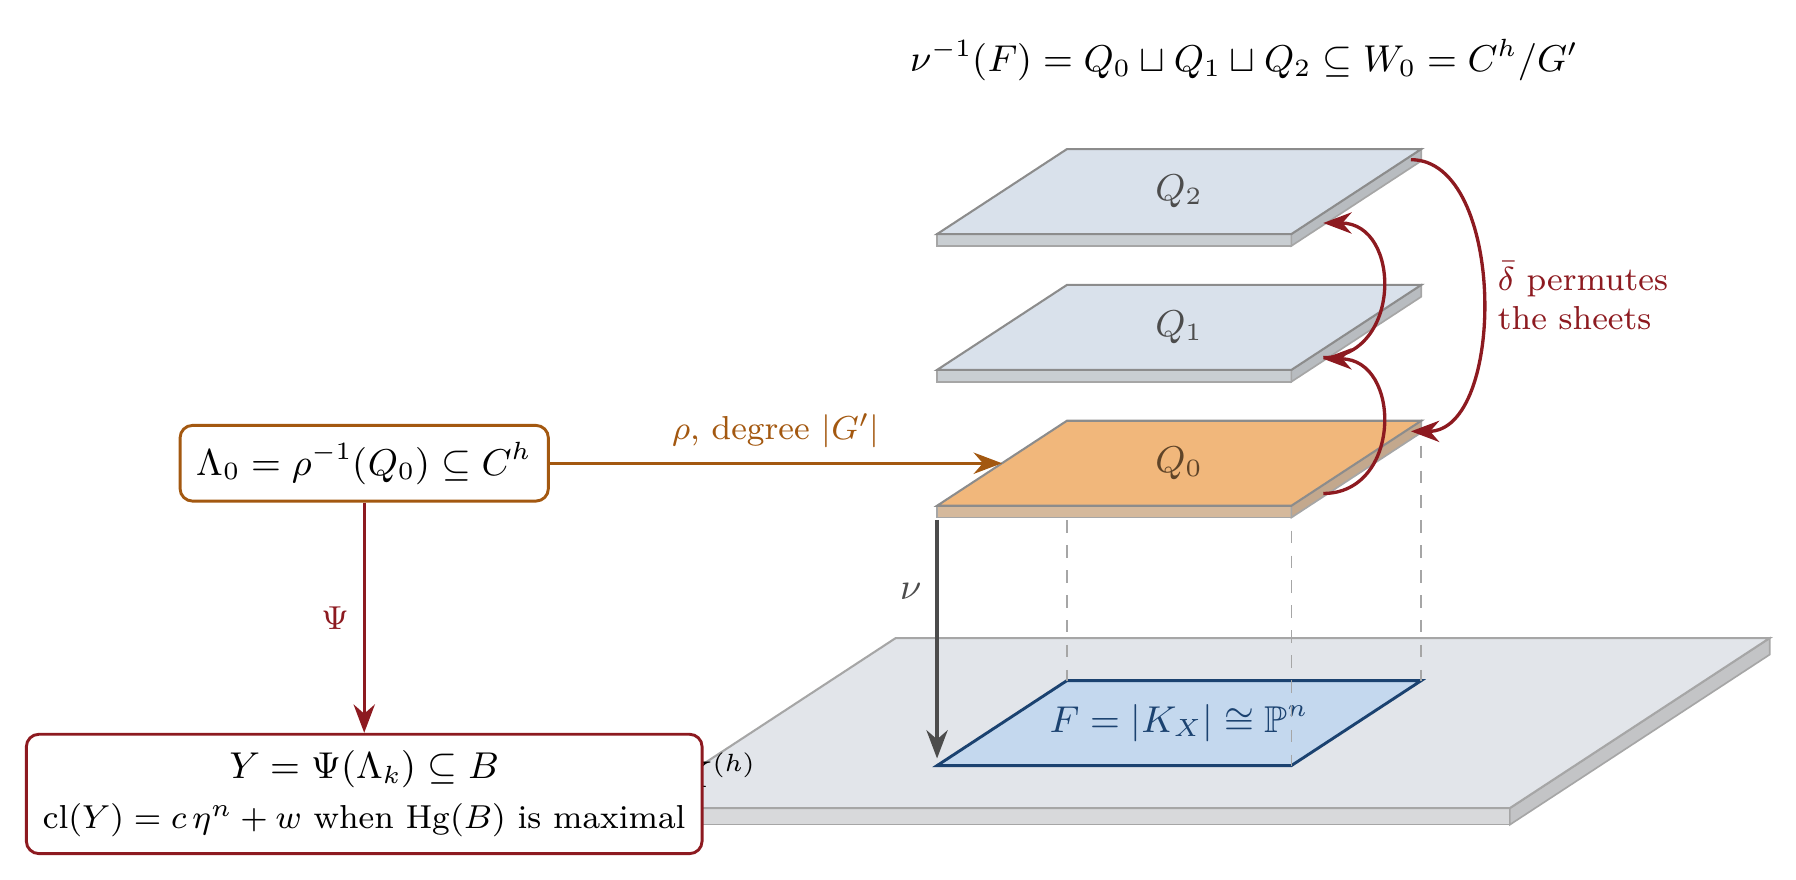
\includegraphics[width=\textwidth]{figures/fig_schoen}
\caption{Schoen's construction. Over the canonical system $F=|K_{X}|$ of
$X$, the \'etale triple cover $\nu\colon W_{0}\to X^{(h)}$ splits into three
sheets, which $\bar\delta$ permutes cyclically. $\Lambda_{0}\subseteq C^{h}$
is the preimage of one sheet, and $Y$ is the image under $\Psi$ of one of
its components (\Cref{thm:E}).}
\label{fig:schoen}
\end{figure}

Fix $c_{0}\in C$ and let
\[
  \Psi\colon C^{h}\to B,\qquad (c_{1},\dots,c_{h})\mapsto
  P\Bigl(\,\sum_{i}(c_{i}-c_{0})\Bigr).
\]

The key input is a computation of cohomology with twisted coefficients.

\begin{lemma}\label{lem:twisted}
Let $\mathcal{L}$ be a nontrivial local system of rank one on $X^{(h)}$.
Then restriction $H^{h}(X^{(h)},\mathcal{L})\to H^{h}(F,\mathcal{L})$ is an
isomorphism, and $H^{h}(F,\mathcal{L})\cong H^{2n}(\PP^{n},\CC)\cong\CC$.
\end{lemma}

\begin{proof}
The fibres of $u$ are projective spaces, so $\mathcal{L}$ is trivial on each
of them, and $\mathcal{M}=u_{*}\mathcal{L}$ is a local system of rank one on
$T=\Pic^{h}(X)$ with $\mathcal{L}=u^{*}\mathcal{M}$.\footnote{By proper base
change the stalk of $u_{*}\mathcal{L}$ at $y$ is $H^{0}(u^{-1}(y),
\mathcal{L})\cong\CC$, so a nonzero section over the fibre extends over
$u^{-1}(D)$ for a small ball $D\ni y$. This set is connected, since $u$ is
proper with connected fibres, and a section of a local system of rank one
over a connected set is determined by its value at one point and vanishes
nowhere unless it is zero. So restriction from $u^{-1}(D)$ to each fibre
over $D$ is an isomorphism, $u_{*}\mathcal{L}$ is locally constant, and
$u^{*}u_{*}\mathcal{L}\to\mathcal{L}$ is an isomorphism on stalks.} It is
nontrivial, because $\mathcal{L}$ is. As a real manifold $T$ is a torus
$(S^{1})^{2g}$, and $\mathcal{M}$ is an exterior product of local systems on
the circles, at least one of them nontrivial; a nontrivial local system of
rank one on a circle has no cohomology, so $H^{*}(T,\mathcal{M})=0$ by the
K\"unneth formula. Let $U=T\setminus\{[K_{X}]\}$. The exact sequence
\[
  \dots\to H^{k}_{c}(U,\mathcal{M})\to H^{k}(T,\mathcal{M})\to
  H^{k}(\{[K_{X}]\},\mathcal{M})\to H^{k+1}_{c}(U,\mathcal{M})\to\dots
\]
gives $H^{1}_{c}(U,\mathcal{M})\cong\CC$ and $H^{k}_{c}(U,\mathcal{M})=0$ for
$k\ne1$. For $M\in U$ Riemann--Roch gives $h^{0}(M)=g-1=n$, so over $U$ the
map $u$ is the projective bundle of a vector bundle of rank $n$
\cite[Chapter~IV]{ACGH85}, and by the Leray--Hirsch theorem
$H^{*}_{c}(u^{-1}(U),\mathcal{L})\cong H^{*}_{c}(U,\mathcal{M})\otimes
H^{*}(\PP^{n-1})$, which vanishes outside the degrees $1,3,\dots,2n-1$. The
exact sequence of the pair $(X^{(h)},F)$,
\[
  H^{h}_{c}(u^{-1}(U),\mathcal{L})\to H^{h}(X^{(h)},\mathcal{L})\to
  H^{h}(F,\mathcal{L})\to H^{h+1}_{c}(u^{-1}(U),\mathcal{L}),
\]
has zero outer terms, since $h=2n$. Finally $\mathcal{L}$ is trivial on the
simply connected $F\cong\PP^{n}$.
\end{proof}

\begin{proof}[Proof of \Cref{thm:E}]
Write $V_{\chi},V_{\bar\chi}\subseteq H^{1}(B,\CC)$ for the eigenspaces of
$\sigma^{*}$ with eigenvalues $\lambda=\chi(\zeta)$ and $\bar\lambda$, and
choose a basis $\bar y_{1},\dots,\bar y_{h}$ of $V_{\bar\chi}$; put
$\bar\omega=\bar y_{1}\wedge\dots\wedge\bar y_{h}$, which spans
$\bigwedge^{2n}V_{\bar\chi}\subseteq W(B)\otimes\CC$.

\emph{Step 1: the pull-back of $\bar\omega$.} Write $\Psi=P'\circ\Xi$, where
$\Xi(c_{1},\dots,c_{h})=\sum_{i}\operatorname{aj}(c_{i})$ and
$\operatorname{aj}(c)=[c-c_{0}]$ is the Abel--Jacobi map. On $H^{1}$ the
pull-back by the addition map $J^{h}\to J$ is the sum of the pull-backs by
the projections, so $\Psi^{*}\bar y_{j}=\sum_{i}p_{i}^{*}\tilde y_{j}$, where
$p_{i}$ is the $i$-th projection of $C^{h}$ and $\tilde y_{j}=
\operatorname{aj}^{*}P'^{*}\bar y_{j}\in H^{1}(C,\CC)$. Since $P'^{*}$ is
injective and $\operatorname{aj}^{*}$ is an isomorphism, both commuting with
$\sigma^{*}$, the $\tilde y_{j}$ are independent and lie in the
$\bar\lambda$-eigenspace of $\sigma^{*}$ on $H^{1}(C,\CC)$. That eigenspace
has dimension $h$, because the invariant part of $H^{1}(C,\CC)$ is
$\pi^{*}H^{1}(X,\CC)$, of dimension $2g$, and the two other eigenspaces are
conjugate; so the $\tilde y_{j}$ form a basis of it. Now
\[
  u:=\Psi^{*}\bar\omega=\prod_{j=1}^{h}\Bigl(\sum_{i=1}^{h}p_{i}^{*}
  \tilde y_{j}\Bigr).
\]
A product $\tilde y_{j}\cup\tilde y_{k}$ lies in the
$\bar\lambda^{2}$-eigenspace of $H^{2}(C,\CC)$, which is zero because
$\sigma$ acts trivially on $H^{2}(C)$ and $\bar\lambda^{2}\ne1$. So in the
expansion only the terms with one factor on each $p_{i}$ survive:
$u=\sum_{s\in S_{h}}\pm\prod_{i}p_{i}^{*}\tilde y_{s(i)}$. By the K\"unneth
formula these terms are linearly independent, and $u\ne0$. Each term is
multiplied by $\bar\lambda^{\sum v_{i}}$ under $(\sigma^{v_{1}}\times\dots
\times\sigma^{v_{h}})^{*}$, and $u$ is symmetric because $\Psi$ is; so $u$
is invariant under $G'$, and $\delta^{*}u=\bar\lambda u$.

\emph{Step 2: restriction to $Q_{0}$.} By transfer, $\rho^{*}$ identifies
$H^{*}(W_{0},\CC)$ with $H^{*}(C^{h},\CC)^{G'}$, so $u=\rho^{*}\bar u$ for a
class $\bar u\ne0$ with $\bar\delta^{*}\bar u=\bar\lambda\bar u$. The
decomposition $\nu_{*}\CC=\bigoplus_{\psi}\mathcal{L}_{\psi}$ into
eigensheaves of $\bar\delta$, indexed by the characters $\psi$ of $\ZZ/3$,
identifies the $\psi(1)$-eigenspace of $\bar\delta^{*}$ on
$H^{*}(W_{0},\CC)$ with $H^{*}(X^{(h)},\mathcal{L}_{\psi})$, compatibly with
restriction to $\nu^{-1}(F)$ and $F$. For $\psi\ne1$ the local system
$\mathcal{L}_{\psi}$ is nontrivial, since $H^{0}(W_{0},\CC)$ is the
invariant line. By \Cref{lem:twisted}, $\bar u$ restricts to a nonzero class
on $\nu^{-1}(F)=Q_{0}\sqcup Q_{1}\sqcup Q_{2}$. As $\bar\delta$ maps $Q_{0}$
isomorphically onto $Q_{t}$ and $\bar u$ is an eigenvector, $\bar u|_{Q_{0}}
=0$ would force $\bar u|_{Q_{t}}=0$ for every $t$. Hence
$\int_{Q_{0}}\bar u\ne0$, and
\[
  \int_{B}\Psi_{*}[\Lambda_{0}]\cup\bar\omega
  =\int_{[\Lambda_{0}]}\rho^{*}\bar u
  =|G'|\int_{Q_{0}}\bar u\ne0.
\]

\emph{Step 3: one component.} The class $\Psi_{*}[\Lambda_{0}]$ is
$\sum_{k}e_{k}\cl(\Psi(\Lambda_{k}))$, the sum over the irreducible
components $\Lambda_{k}$ of $\Lambda_{0}$ on which $\Psi$ is generically
finite, with $e_{k}$ the degree of $\Lambda_{k}\to\Psi(\Lambda_{k})$. By Step
2 one of them, say $Y=\Psi(\Lambda_{k})$, satisfies $\int_{B}\cl(Y)\cup
\bar\omega\ne0$. It is irreducible of dimension $n$. Since $W(B)\otimes\CC$
is spanned by $\bar\omega$ and its conjugate, $\cl(Y)$ pairs nontrivially
with $W(B)$.

\emph{Step 4: the shape of the class.} If $\Hg(B)=\SU(V,H)$, then
\Cref{prop:hodgering} gives $\cl(Y)=c\,\eta^{n}+w$ with $c\in\QQ$ and $w\in
W(B)$. Since $\eta^{n}\cup\bar\omega=0$, Step~3 gives $w\ne0$. Since
$\eta^{n}\cup w=0$,
\[
  c\int_{B}\eta^{2n}=\int_{B}\cl(Y)\cup\eta^{n}=\deg_{\eta}Y>0,
\]
so $c>0$. The last assertion of \Cref{thm:E} is \Cref{cor:schoensemireg}
below.
\end{proof}

\begin{corollary}[Schoen \cite{Sch88}]\label{cor:schoen}
For every \'etale cyclic triple cover of a curve of genus at least three,
the Prym variety $B$ is Weil-algebraic.
\end{corollary}

\begin{proof}
If $B$ has maximal Hodge group, $w=\cl(Y)-c\,\eta^{n}$ is a nonzero
algebraic class in $W(B)$, and $B$ is Weil-algebraic. By
\Cref{lem:prym}(c) this covers every $(X,L)$ outside a countable union of
proper closed subsets $Z_{i}$ of a smooth connected base $T$ over which, after a finite \'etale
base change, the Prym varieties form a polarized abelian scheme with a
trivial local system of Weil planes.\footnote{Take for $T$ a connected
component of a finite \'etale cover of the moduli space of curves of genus
$g$ with level-$3$ structure, on which $L$ is the section given by a fixed
nonzero vector of $(\ZZ/3)^{2g}$. The monodromy acts on the Weil planes
through the determinant, which takes values in the roots of unity of
$\cO_{K}$, so it becomes trivial on a finite cover.} The proof of
\Cref{lem:sigmaclosed} shows that the locus where the Weil classes have
algebraic representatives of degree at most $d$ is Zariski closed in $T$.
These countably many closed sets, together with the $Z_{i}$, cover $T$, so
by the Baire category theorem one of them has interior. It is not a $Z_{i}$,
so it is one of the degree-$d$ loci, and it equals $T$.
\end{proof}

\begin{corollary}\label{cor:schoensemireg}
Suppose that for one $(X,L)$ of genus $n+1\ge3$ with maximal Hodge group the
subvariety $Y$ of \Cref{thm:E} is semiregular. Then every abelian variety of
split Weil type for $\QQ(\sqrt{-3})$ of dimension $2n$ is Weil-algebraic.
\end{corollary}

\begin{proof}
The sheaf $\cO_{Y}$ has $\ch_{k}(\cO_{Y})=0$ for $k<n$ and $\ch_{n}(\cO_{Y})=
\cl(Y)=c\,\eta^{n}+w$ with $w\ne0$ \cite[Chapter~15]{Ful98}; for $k>n$ the
class $\ch_{k}(\cO_{Y})$ is algebraic, hence a multiple of $\eta^{k}$ by
\Cref{prop:hodgering}. By \Cref{lem:prym}(b), $B$ is a member of a split
Weil family $S$ as in \Cref{ssec:weilfamilies}, and \Cref{prop:semireg}
gives $\Sigma=S$. Every abelian variety of split Weil type for $K$ of
dimension $2n$ is $K$-isogenous to a member of $S$,\footnote{Two split
hermitian forms of the same dimension are isometric, being orthogonal sums
of hyperbolic planes. An isometry carries the complex structure of the
first variety to a point of the symmetric domain of the second form, and
the two lattices are commensurable in the same $K$-vector space.} and a
$K$-isogeny $f$ carries Weil planes to Weil planes and algebraic classes to
algebraic classes in both directions, through $f^{*}$ and
$(\deg f)^{-1}f_{*}$.
\end{proof}

\subsection{Transfer by correspondences}\label{ssec:transfer}
Schoen's cycles reach a family of dimension $3n$ inside one of dimension
$n^{2}$. One way to spread them is to carry the Weil classes to other
varieties by correspondences. This gives a theorem, but a count of
dimensions shows that it cannot reach the general member by itself.

\begin{lemma}\label{lem:twothree}
Let $B$, $A_{1}$ and $A_{2}$ be of Weil type for $K$, of dimensions
$2(m_{1}+m_{2})$, $2m_{1}$ and $2m_{2}$, and let $f\colon B\to A_{1}\times
A_{2}$ be an isogeny that commutes with $\cO_{K}$.
\begin{enumerate}[label=\textup{(\alph*)}]
\item $f^{*}$ carries a plane in $W(A_{1})\otimes W(A_{2})$ onto $W(B)$;
over $\CC$ the plane is spanned by $\omega_{1}\otimes\omega_{2}$ and
$\bar\omega_{1}\otimes\bar\omega_{2}$, where $\omega_{i}$ spans
$\bigwedge^{2m_{i}}V_{\chi}(A_{i})$.
\item If two of $B$, $A_{1}$, $A_{2}$ are Weil-algebraic, so is the third.
\end{enumerate}
\end{lemma}

\begin{proof}
As in the proof of \Cref{cor:schoensemireg}, we may take $B=A_{1}\times
A_{2}$. Then $V_{\chi}(B)=V_{\chi}(A_{1})\oplus V_{\chi}(A_{2})$, and the top
exterior power of a sum is the tensor product of the top exterior powers;
this is~(a). If $A_{1}$ and $A_{2}$ are Weil-algebraic, every class in
$W(A_{1})\otimes W(A_{2})$ is a sum of products $\pr_{1}^{*}\alpha_{1}\cup
\pr_{2}^{*}\alpha_{2}$ of algebraic classes, so $B$ is Weil-algebraic by~(a).
Suppose that $B$ and $A_{2}$ are Weil-algebraic. On $A_{2}$ we have
$\omega_{2}\cup\omega_{2}=0$, since $\bigwedge^{4m_{2}}V_{\chi}(A_{2})=0$,
while $p=\int\omega_{2}\cup\bar\omega_{2}\ne0$, since
$\bigwedge^{2m_{2}}V_{\chi}\otimes\bigwedge^{2m_{2}}V_{\bar\chi}$ is the top
exterior power of $H^{1}(A_{2},\CC)$; and $p$ is real, because classes of
even degree commute. Nonzero rational classes $x\in W(B)$ and $\gamma\in
W(A_{2})$ have the form $x=s\,\omega_{1}\otimes\omega_{2}+\bar s\,
\bar\omega_{1}\otimes\bar\omega_{2}$ and $\gamma=t\,\omega_{2}+\bar t\,
\bar\omega_{2}$ with $s,t\ne0$. The class
\[
  \pr_{1*}\bigl(x\cup\pr_{2}^{*}\gamma\bigr)=p\,\bigl(s\bar t\,\omega_{1}+
  \bar st\,\bar\omega_{1}\bigr)
\]
is rational, algebraic, nonzero, and lies in $W(A_{1})$.
\end{proof}

\begin{lemma}\label{lem:EEbar}
Let $K$ be any imaginary quadratic field, $E$ an elliptic curve with complex
multiplication by $\cO_{K}$, and $\bar E$ the same curve with $\cO_{K}$
acting through complex conjugation. For $k\ge1$ the variety $E^{k}\times
\bar E^{k}$, with the product polarization, is of split Weil type, and its
Weil classes are polynomials in divisor classes.
\end{lemma}

\begin{proof}
On $H_{1}(E,\QQ)=K$ the polarization is $\operatorname{Tr}_{K/\QQ}(f\,x\bar
y)$ for some $f\in K$ with $\bar f=-f$, so its hermitian form is
$x\bar y$. For $\bar E$ the $K$-structure is conjugated, and the same
Riemann form is $\operatorname{Tr}_{K/\QQ}(f\cdot(-\bar xy))$, with
hermitian form $-\bar xy$. So the form of $E^{k}\times\bar E^{k}$ is
$\operatorname{diag}(1,\dots,1,-1,\dots,-1)$, for which the vectors
$e_{i}+e_{k+i}$ span an isotropic subspace of dimension $k$, and both
embeddings of $K$ occur $k$ times on $H^{1,0}$. With coordinates
$z_{1},\dots,z_{2k}$ on the factors, $V_{\chi}$ is spanned by $dz_{1},\dots,
dz_{k}$ and $d\bar z_{k+1},\dots,d\bar z_{2k}$, so up to sign
$\omega_{\chi}=\bigwedge_{i=1}^{k}(dz_{i}\wedge d\bar z_{k+i})$. Each factor
is a class of type $(1,1)$ on $E\times\bar E\cong E\times E$, whose
N\'eron--Severi group has rank $4=h^{1,1}$ because $E$ has complex
multiplication; so it is a complex combination of divisor classes, and so
are $\omega_{\chi}$ and its conjugate.
\end{proof}

\begin{theorem}\label{thm:transfer}
Let $A$ be an abelian variety of Weil type for $K=\QQ(\sqrt{-3})$, of
dimension $2m\ge2$, on which $\cO_{K}$ acts. There are a smooth curve
$C\subseteq A$, stable under $\zeta$ and with $\zeta$ acting freely on it, so
that $C\to X=C/\zeta$ is an \'etale cyclic triple cover of a curve of some
genus $g\ge m+1$; an abelian variety $A'$ of Weil type of dimension
$2(g-1-m)$; and an isogeny commuting with $\cO_{K}$ between the Prym variety
of $C\to X$ and $A\times A'$. For every such curve, $A$ is Weil-algebraic if
and only if $A'$ is.
\end{theorem}

\begin{proof}
\emph{The curve.} The automorphism $\zeta$ has finitely many fixed points,
the kernel of the isogeny $1-\zeta$. Let $\mathcal{N}$ be ample on $A$. The bundle $\mathcal{N}'=\mathcal{N}\otimes\zeta^{*}\mathcal{N}\otimes
\zeta^{2*}\mathcal{N}$ is isomorphic to its pull-back by $\zeta$, so it carries a linearization for the
cyclic group generated by $\zeta$;\footnote{Choose an isomorphism
$\phi\colon\zeta^{*}\mathcal{N}'\to\mathcal{N}'$. The composite of $\phi$,
$\zeta^{*}\phi$ and $\zeta^{2*}\phi$ is an automorphism of $\mathcal{N}'$,
hence a scalar $c$, and $c^{-1/3}\phi$ is a linearization.} its cube
descends to an ample line bundle $\bar{\mathcal{M}}$ on the normal quotient
$q\colon A\to A/\zeta$, since the stabilizers, of order dividing three, act
trivially on its fibres. For $k$ large, $2m-1$ general members $D_{i}$ of
$|\bar{\mathcal{M}}^{k}|$ meet in a smooth irreducible curve $X$ that avoids
the images of the fixed points, by Bertini's theorem. Then $C=q^{-1}(X)$ is
\'etale over $X$, hence smooth, and it is the complete intersection of the
ample divisors $q^{*}D_{i}$, hence connected. Schoen observes the existence
of such curves in \cite[\S3]{Sch88}.

\emph{The surjection.} By the Lefschetz hyperplane theorem, restriction
$H^{1}(A,\QQ)\to H^{1}(C,\QQ)$ is injective, so the homomorphism
$\alpha\colon J(C)\to A$ induced by the inclusion is surjective; it commutes
with $\zeta$. Since $1+\zeta+\zeta^{2}=0$ in $\cO_{K}$, $\alpha N=0$ and
$\alpha P=3\alpha$. So $\alpha$ maps the Prym variety $B=P(J(C))$ onto $A$,
and $g-1\ge m$.

\emph{The complement.} Let $A'$ be the connected component of the kernel of
$\alpha|_{B}$ and $A''$ its complement in $B$ for the induced polarization.
Both are stable under $\sigma$, which preserves the polarization, so
$\cO_{K}$ acts on them, and $A''\to A$ and $A'\times A''\to B$ are isogenies
commuting with $\cO_{K}$. By \Cref{lem:prym}(a) both embeddings of $K$ occur
$g-1$ times on $H^{1,0}(B)$, and they occur $m$ times on $H^{1,0}(A)$; so
they occur $g-1-m$ times on $H^{1,0}(A')$, and $A'$ is of Weil type.

\emph{The equivalence.} $B$ is Weil-algebraic by \Cref{cor:schoen}, and
\Cref{lem:twothree}(b) gives the equivalence.
\end{proof}

\begin{corollary}\label{cor:transfer}
$A$ is Weil-algebraic as soon as, for one curve as in \Cref{thm:transfer},
the complement $A'$ is $K$-isogenous to a product of Weil-algebraic
varieties, such as Prym varieties of \'etale cyclic triple covers
(\Cref{cor:schoen}), abelian surfaces of Weil type (\Cref{thm:lef11}), and
the varieties $E^{k}\times\bar E^{k}$ (\Cref{lem:EEbar}).
\end{corollary}

\begin{proof}
Products of Weil-algebraic varieties are Weil-algebraic by
\Cref{lem:twothree}(b), and \Cref{thm:transfer} applies.
\end{proof}

When $g-1=m$ the complement is zero and $A$ is $K$-isogenous to a Prym
variety. For larger $g$ the theorem trades the Weil classes of $A$ for those
of $A'$, and since curves of higher degree give complements of every size,
one might hope to choose the curve so that $A'$ is of a known kind. The
count below says that for $m\ge4$ this hope fails at the general member
unless an unexpected intersection occurs.

\begin{remark}\label{rem:count}
Pryms of \'etale triple covers of curves of genus $m+k+1$ form a family of
dimension $3(m+k)$ inside the Weil family of dimension $(m+k)^{2}$. The
varieties $K$-isogenous to $A\times A'$, with $A$ in the family of dimension
$m^{2}$ and $A'$ in a family of dimension $f$, form a subvariety of dimension
$m^{2}+f$. For $A$ to be general the two must meet in dimension at least
$m^{2}$, which needs $3(m+k)+f\ge(m+k)^{2}$ unless they meet in excess
dimension. Products of the varieties of \Cref{cor:transfer} of total
dimension $2k$ have at most $3k$ moduli, and $3(m+k)+3k<(m+k)^{2}$ for every
$k\ge0$ once $m\ge4$. For $m=3$ only $k=0$ passes, the Prym locus itself, and
for $m=2$ exactly $k\le2$ pass. So \Cref{cor:transfer} reaches only a meagre
part of the family once $m\ge4$, unless the Prym locus meets these product
loci in excess dimension, as Schoen anticipated \cite[\S3]{Sch88}. This is a
count, not a proof that no such intersection exists.
\end{remark}

\subsection{Where it stops}\label{ssec:whereitstops}
Everything on the Weil route now rests on one question.

\begin{question}\label{q:schoen}
Let $n\ge4$ and let $(X,L)$ be very general of genus $n+1$. Is the subvariety
$Y\subseteq B$ of \Cref{thm:E} semiregular?
\end{question}

A positive answer forces $Y$ to deform with $B$ to first order along all
$n^{2}$ directions of the Weil family, and not only along the $3n$
directions of the Prym locus; so it asks for $n^{2}-3n$ unexpected first
order deformations. We have not been able to decide the question, and the
closest analogue points the other way.

The Abel--Jacobi curve $C\subseteq J(C)$ of a curve of genus $g\ge4$ is
built from the same map as $Y$. Its class $\theta^{g-1}/(g-1)!$ is a Hodge
class on every principally polarized abelian variety. Yet by the criterion
of Matsusaka and Ran \cite{Mat59,Ran81} a curve with this class exists only
on Jacobians and products of Jacobians, which form a proper subvariety of the
moduli space $\mathcal{A}_{g}$. So the curve does not deform in the
directions normal to the Jacobian locus, and by \Cref{thm:bf} it is not
semiregular. The number of those directions is classical. The tangent space
to $\mathcal{A}_{g}$ at $J(C)$ is dual to $\operatorname{Sym}^{2}H^{0}(K_{C})$,
the tangent space to the Jacobian locus is dual to $H^{0}(2K_{C})$, and by
Max Noether's theorem the multiplication map between them is surjective for
non-hyperelliptic $C$, with kernel the space $I_{2}$ of quadrics containing
the canonical curve. So the Jacobian locus has codimension
\[
  \dim I_{2}=\binom{g+1}{2}-(3g-3)=\frac{(g-2)(g-3)}{2}
\]
at $J(C)$. Schoen's subvariety is the analogue one step up, built from the
fibre of the Abel--Jacobi map over the canonical class, and the
corresponding codimension, that of the Prym locus in the Weil family, is
$n^{2}-3n$. Nothing in the construction of $Y$ moves it off the Prym locus.
This is an analogy and not a proof.

Nor can a branched cover take the place of the \'etale one, because
branching does not enlarge the Prym locus enough.

\begin{proposition}\label{prop:branched}
Let $\pi\colon C\to X$ be a cyclic triple cover of a curve of genus $q$,
branched at $r$ points, with covering automorphism $\sigma$, and let its
Prym variety, the image of $3-N$ on $J(C)$ with $N=1+\sigma+\sigma^{2}$,
have dimension $2n$. Then $2q+r=2n+2$, and the covers with these
invariants form finitely many families, each of dimension $q+2n-1\le3n$,
with equality only for \'etale covers of curves of genus $n+1$. In
particular, for $n\ge4$ a very general member of the split Weil family of
$K$ in dimension $2n$ is not $K$-isogenous to the Prym variety of any cyclic
triple cover, \'etale or branched.
\end{proposition}

\begin{proof}
Since $3$ is prime, every branch point is totally ramified, and the
Riemann--Hurwitz formula $2g(C)-2=3(2q-2)+2r$ gives $g(C)=3q-2+r$. The
invariant part of $H^{0}(C,K_{C})$ under $\sigma^{*}$ is
$\pi^{*}H^{0}(X,K_{X})$, of dimension $q$, and as in the proof of
\Cref{lem:prym}(a) the space $H^{1,0}$ of the Prym variety is the sum of the
two other eigenspaces. So the Prym variety has dimension $g(C)-q=2q-2+r$,
and $2q+r=2n+2$. Given $X$ and the $r$ branch points, the cover corresponds
to a surjection from the fundamental group of the punctured curve onto
$\ZZ/3$, and there are finitely many of these. So the covers form finitely
many families, of dimension $3q-3+r$ when $q\ge2$, $r$ when $q=1$, and
$r-3$ when $q=0$; by $r=2n+2-2q$ each of these equals $q+2n-1$. As $r\ge0$,
$q\le n+1$, so the dimension is at most $3n$, and it equals $3n$ exactly
when $q=n+1$ and $r=0$.

The Prym varieties of each family form the image of a variety of
dimension at most $3n$ in the moduli space, and the $K$-isogenies of a given
degree carry it to finitely many subvarieties of at most the same
dimension. The members of the split
Weil family that are $K$-isogenous to such a Prym variety therefore lie in a
countable union of subvarieties of dimension at most $3n$, which for
$n\ge4$ is less than $n^{2}$.
\end{proof}

The analogy with the Abel--Jacobi curve can be tested on $B$ itself, in
dimension one. Following Lange and Ortega \cite{LO11}, call
\[
  \psi\colon C\to B,\qquad \psi(c)=(1-\sigma)(c-c_{0}),
\]
the \emph{Abel--Prym map}. As $P=(1-\sigma)(1-\sigma^{2})$, the restriction
of $\Psi$ to one factor is $(1-\sigma^{2})\circ\psi$, and $1-\sigma^{2}$ is
an isogeny of $B$. Put $V_{j}=H^{0}(X,K_{X}\otimes L^{j})$, so that
$H^{0}(C,K_{C})=V_{0}\oplus V_{1}\oplus V_{2}$ as in the proof of
\Cref{lem:prym}(a), and let
\[
  \mu_{L}\colon V_{1}\otimes V_{2}\longrightarrow H^{0}(X,K_{X}^{\otimes2})
\]
be multiplication of sections, through an isomorphism $L^{3}\cong\cO_{X}$.
A first-order deformation of $X$ with Kodaira--Spencer class $u\in
H^{1}(X,T_{X})$ carries the \'etale cover along with it, uniquely, and with
it $J(C)$, $\sigma$ and $B$. Write $d\mathcal{P}(u)\in H^{1}(B,T_{B})$ for the
Kodaira--Spencer class of the resulting deformation of $B$. Lange and Ortega
identify the dual of $d\mathcal{P}$ with a multiplication map
\cite{LO11}, and we derive the form of this that we need in the proof
below.

\begin{proposition}\label{prop:abelprym}
Let $v\in H^{1}(B,T_{B})$ be the Kodaira--Spencer class of a first-order
deformation $\mathcal{B}$ of $B$ to which $\sigma$ extends. Then $\psi$
extends to a morphism into $\mathcal{B}$ from some first-order deformation of
$C$ if and only if $v$ lies in the image of $d\mathcal{P}$, and this image has
dimension $\operatorname{rk}\mu_{L}\le3n$. Suppose moreover that $n\ge4$,
that $B$ has maximal Hodge group, and that $S$ is a split Weil family
containing $B$ (\Cref{lem:prym}(b)). Then the tangent vectors to $S$ at $B$ along which
$\psi$ extends form a subspace of codimension at least $n^{2}-3n$, although
$\psi_{*}[C]$ is a rational multiple of $\eta^{2n-1}$, whose flat continuation
is algebraic on every member of $S$.
\end{proposition}

\begin{proof}
All deformations are over $\operatorname{Spec}\CC[t]/(t^{2})$. Suppose that
$\psi$ extends to $\psi_{t}\colon\mathcal{C}\to\mathcal{B}$, where
$\mathcal{C}$ is a deformation of $C$ with class $w\in H^{1}(C,T_{C})$. Cover
$C$ and $B$ by affine open sets $U_{i}$ and $W_{i}$ with $\psi(U_{i})\subseteq
W_{i}$ over which $\mathcal{C}$ and $\mathcal{B}$ are trivial, with
transition automorphisms $1+t\theta_{ij}$ and $1+t\xi_{ij}$, where
$(\theta_{ij})$ and $(\xi_{ij})$ are cocycles of vector fields representing
$w$ and $v$. On $U_{i}$ the map $\psi_{t}$ is $\psi+ts_{i}$ for a section
$s_{i}$ of $\psi^{*}T_{B}$, and compatibility on $U_{i}\cap U_{j}$ reads
$s_{j}-s_{i}=\psi^{*}\xi_{ij}-d\psi(\theta_{ij})$ \cite{Hor74}. Hence
\begin{equation}\label{eq:horikawa}
  \psi^{*}v=H^{1}(d\psi)(w)\quad\text{in }H^{1}(C,\psi^{*}T_{B}),
\end{equation}
where $d\psi\colon T_{C}\to\psi^{*}T_{B}$ is the differential.

We compute both sides by Serre duality. The bundle $T_{B}$ is trivial with
fibre $T_{0}B$, and $\psi^{*}$ identifies $H^{0}(B,\Omega^{1}_{B})$ with
$V_{-}=V_{1}\oplus V_{2}$. Indeed, since $(1-\sigma)N=0$, the pull-back by
$1-\sigma\colon J\to B$ maps $H^{1,0}(B)$ injectively into the sum of the
nontrivial eigenspaces of $\sigma^{*}$ on $H^{1,0}(J)$, which has dimension
$2n=\dim B$, and the Abel--Jacobi map identifies this sum with $V_{-}$. So $H^{1}(C,\psi^{*}T_{B})=H^{1}(C,\cO_{C})\otimes T_{0}B$ is
dual to $H^{0}(C,K_{C})\otimes V_{-}$, and $H^{1}(C,T_{C})$ is dual to
$H^{0}(C,K_{C}^{\otimes2})$. The dual of $d\psi$ is evaluation
$\cO_{C}\otimes V_{-}\to K_{C}$, so the dual of $H^{1}(d\psi)$ is
multiplication
\[
  m\colon H^{0}(C,K_{C})\otimes V_{-}\longrightarrow
  H^{0}(C,K_{C}^{\otimes2})
\]
\cite{LO11}. Thus \eqref{eq:horikawa} says that $\psi^{*}v$, as a
linear form on $H^{0}(C,K_{C})\otimes V_{-}$, is $w\circ m$.

Now use $\sigma$. We have $\psi\sigma=t_{a}\sigma\psi$, where $t_{a}$ is the
translation by $a=(1-\sigma)(\sigma c_{0}-c_{0})$. Translations act trivially
on $H^{1}(B,\cO_{B})$ and on $T_{0}B$, so $\psi^{*}$ commutes with the actions
of $\sigma$, and $m$ is equivariant. As $\sigma$ extends to $\mathcal{B}$, the
class $v$ is invariant, and so is the form $\psi^{*}v$; an invariant form
vanishes on every eigenspace of $\sigma$ with an eigenvalue other than $1$.
The automorphism $\sigma^{*}$ acts on $V_{j}$ by $\kappa^{j}$ for a primitive
cube root of unity $\kappa$, so the invariant part of
$H^{0}(C,K_{C})\otimes V_{-}$ is $E=(V_{1}\otimes V_{2})\oplus(V_{2}\otimes
V_{1})$. Since $\pi_{*}K_{C}^{\otimes2}=K_{X}^{\otimes2}\otimes\pi_{*}\cO_{C}$,
the map $m$ sends $E$ to $H^{0}(C,K_{C}^{\otimes2})^{\sigma}=\pi^{*}H^{0}(X,
K_{X}^{\otimes2})$, by $(x,y)\mapsto\pi^{*}M(x,y)$ with
$M(x,y)=\mu_{L}(x+\tau y)$, where $\tau\colon V_{2}\otimes V_{1}\to
V_{1}\otimes V_{2}$ is the transposition. So $\psi^{*}v$ is determined by its
restriction to $E$, which by \eqref{eq:horikawa} is $f\circ M$, where $f$ is
the linear form $q\mapsto\langle w,\pi^{*}q\rangle$ on
$H^{0}(X,K_{X}^{\otimes2})$, that is, an element of $H^{1}(X,T_{X})$.

Apply this to the deformation of $B$ induced by $u\in H^{1}(X,T_{X})$. The
deformation of $C$ has class $\pi^{*}u$, and $\psi$ extends after $c_{0}$ is
extended to a section. Since $\pi$ has degree $3$, $\langle\pi^{*}u,
\pi^{*}q\rangle=3\langle u,q\rangle$, so the restriction of
$\psi^{*}d\mathcal{P}(u)$ to $E$ is $3\,u\circ M$. Returning to $v$, the
invariant forms $\psi^{*}v$ and $\psi^{*}d\mathcal{P}(f/3)$ agree on $E$,
hence everywhere. The map $\psi^{*}$ on $H^{1}(B,T_{B})=H^{1}(B,\cO_{B})
\otimes T_{0}B$ is injective, since on $H^{1}(B,\cO_{B})$ it is the complex
conjugate of the injective map on $H^{0}(B,\Omega^{1}_{B})$. So
$v=d\mathcal{P}(f/3)$. Conversely, if $v=d\mathcal{P}(u)$, then $\mathcal{B}$
is isomorphic to the deformation induced by $u$, since first-order
deformations are determined by their Kodaira--Spencer classes, and $\psi$
extends. Finally $d\mathcal{P}(u)=0$ exactly when $u\circ M=0$, that is, when
$u$ vanishes on the image of $\mu_{L}$; so $d\mathcal{P}$ has rank
$\operatorname{rk}\mu_{L}\le h^{0}(X,K_{X}^{\otimes2})=3g-3=3n$.

For the last assertion, the element $\zeta\in\cO_{K}$ acts on the abelian
scheme over $S$ as $\sigma$ on $B$, so the Kodaira--Spencer map
$T_{S,B}\to H^{1}(B,T_{B})$ has invariant image. It is injective, because $S$
is locally isomorphic to the symmetric domain $\cD$, the period map of the
family lifts to the inclusion of $\cD$ in the period domain, and the
differential of the period map is the Kodaira--Spencer map followed by the
isomorphism $H^{1}(B,T_{B})\cong\operatorname{Hom}(H^{1,0}(B),
H^{0,1}(B))$ \cite[Chapter~10]{Voi02b}. So the tangent vectors along which
$\psi$ extends form a subspace of dimension at most $3n$ in the
$n^{2}$-dimensional space $T_{S,B}$. By \Cref{prop:hodgering},
$\psi_{*}[C]\in\Hdg^{2n-1}(B)=\QQ\,\eta^{2n-1}$.
\end{proof}

So the curve $\psi(C)$, whose class stays algebraic on the whole family,
moves with $B$ only along the Prym locus. When $X$ has Clifford index at
least $2$, as a very general curve of genus at least $5$ does
\cite[Chapter~V]{ACGH85}, the map $\psi$ is a closed embedding
\cite{LO11}, and then, for $n\ge4$ and $B$ with maximal Hodge group, the
curve $\psi(C)$ is not semiregular. Otherwise \Cref{thm:bf} would extend
$\cO_{\psi(C)}$ along every tangent vector of $S$; a first-order deformation of $\cO_{\psi(C)}$ is locally
generated by one section, so it is a line bundle on the subscheme defined by
its annihilator, which is a first-order deformation of $\psi(C)$ and so
carries an extension of $\psi$, against \Cref{prop:abelprym}.

This makes the analogy precise on $B$, but it does not decide
\Cref{q:schoen}. The subvariety $Y$ is the image of the $n$-dimensional
variety $\Lambda_{k}$, and the same computation for $\Psi$ on $\Lambda_{k}$
would need the cohomology of a resolution of $\Lambda_{k}$, which we have not
determined. Nor does the rigidity of a curve predict that of the image of a
higher symmetric product: the theta divisor of a Jacobian is the image of the
$(g-1)$-st symmetric product of the curve under the Abel--Jacobi map, and it
deforms with every principally polarized abelian variety.

A weaker hypothesis would do if the semiregularity theorem were sharper.
Markman asks whether \Cref{thm:bf} holds when $\sigma_{\mathcal{E}}$ is
injective only on the image of the evaluation map from the second Hochschild
cohomology $HH^{2}(Z)$ to $\operatorname{Ext}^{2}(\mathcal{E},\mathcal{E})$
\cite[Question~11.4]{Mar25b}. A positive answer would replace the
semiregularity of $\cO_{Y}$ in \Cref{cor:schoensemireg} by injectivity of
$\sigma_{\cO_{Y}}$ on that image, a condition that involves only the
deformations of $B$ and of its category of sheaves. For a general imaginary
quadratic field, cycles representing Weil classes at members with maximal
Hodge group are known in dimension four, and for split forms in dimension
six \cite{Mar25a}. For nonsplit forms in dimension six, and in dimension
$2n\ge8$ for fields other than $\QQ(\sqrt{-3})$ and $\QQ(\sqrt{-1})$, we
know of none, so the route has nothing to deform.
